\documentclass[12pt]{article}
\usepackage{amssymb,amsmath,graphicx,mathtools}
\usepackage{listings}
\usepackage[margin=0.75in]{geometry}
\parindent 16 pt
\usepackage{fancyhdr}
\pagestyle{fancy}
\fancyhead[R]{Swupnil Sahai}
\fancyhead[C]{03/21/16}
\fancyhead[L]{Kernel Model}
\DeclarePairedDelimiter\ceil{\lceil}{\rceil}
\DeclarePairedDelimiter\floor{\lfloor}{\rfloor}

\lstset{
    language=R,
    basicstyle=\scriptsize\ttfamily,
    stepnumber=1,
    numbersep=5pt,
    showspaces=false,
    showstringspaces=false,
    showtabs=false,
    frame=single,
    tabsize=2,
    captionpos=b,
    breaklines=true,
    breakatwhitespace=false,
    escapeinside={},
    keywordstyle={},
    morekeywords={}
    }

\begin{document}

% CUSTOM SHORTCUTS

\def\ci{\perp\!\!\!\perp}
\def\ex{\mathbb{E}}
\def\prob{\mathbb{P}}
\def\ind{\mathbb{I}}
\def\grad{\triangledown}
\def\bigo{\mathcal{O}}

%MODEL FORUMLATION
\subsection*{Motivation}
The previous model using a mixing matrix had bias/variance and identifiability issues because the parameters lacked constraints (other than the rows summing to 1). In an effort to fix this issue, we've now built a model with more structure and far fewer parameters.

\subsection*{Formulation}
We are still using a negative binomial formulation but the expression for the mean has been modified to express mixing using a Gaussian kernel:

$$ y_{ik} \sim \text{NegBin}(\omega_k \mu_{ik}, \omega_k)
\hspace{20 pt} E(y_{ik}) = \mu_{ik} 
\hspace{20 pt} Var(y_{ik}) = \mu_{ik} + \frac{\mu_{ik}}{\omega_k}$$

\noindent  Now let $a_i \in (-\infty,\infty)$ and $g_i \in \{M,F\}$ denote the age and gender of ego $i$, respectively, while we let $g_k$ denote the gender of alter name $k$. Then we can derive the mean expression as follows:

$$ \mu_{ik} = N_i p(k, g_k | a_i,g_i)
= N_i \int_s p(k, s, g_k | g_i, a_i) ds
= N_i \int_s p(k | s, g_k, g_i, a_i) p(s, g_k | g_i, a_i) ds $$
$$ = N_i \int_s p(k | s, g_k) p(s | g_k, g_i, a_i) p(g_k | g_i, a_i) ds
= N_i \int_s p(k | s, g_k) p(s | g_k, g_i, a_i) p(g_k | g_i) ds $$
$$ = N_i p_{g_ig_k} \int_s p(k | s, g_k) \mathcal{K}_{g_ig_k}(a_i, s) ds$$

\noindent where the kernel is parametrized as:

$$ \mathcal{K}_{g_ig_k}(a_i, a_j) = \frac{1}{\sqrt{2\pi\lambda_{g_ig_k}}} e^{-\frac{(a_i-a_j)^2}{2\lambda_{g_ig_k}}} $$

%SIMPLIFICATION%
\subsection*{Simplification Options}
1. If we assume $p(k | s, g_k) \sim \mathcal{N}(\mu_{k}, \sigma_{k})$, we can simplify the integral in the expression of $\mu_{ik}$ using the product of unconstrained normals:
$$ \int \mathcal{K}_{g_ig_k}(a_i, s) p(k | s, g_k) ds
=  \int_{-\infty}^{\infty} \frac{1}{\sqrt{2\pi\lambda_{g_ig_k}}} e^{-\frac{(a_i-s)^2}{2\lambda_{g_ig_k}}} \frac{1}{\sqrt{2\pi}\sigma_{k}} e^{-\frac{(s-\mu_k)^2}{2\sigma_{k}^2}}ds 
= \frac{ e^{-\frac{(a_i-\mu_k)^2}{2(\lambda_{g_ig_k}+\sigma_{k}^2)}} }{\sqrt{2\pi(\lambda_{g_ig_k} + \sigma_{k}^2)}} $$

\noindent We can then reformulate the expectation as such:
$$\mu_{ik} =
\frac{N_i p_{g_ig_k}}{\sqrt{2\pi(\lambda_{g_ig_k} + \sigma_{k}^2)}} e^{-\frac{(a_i-\mu_{k})^2}{2(\lambda_{g_ig_k}+\sigma_{k}^2)}} 
$$

\noindent 2. An alternative simplification is to refactorize $p(k | s, g_k) = \frac{p(s | k, g_k) p(k, g_k)}{p(s, g_k)}$ and then assume that $p(s | k, g_k) \sim \mathcal{N}(\mu_{k}, \sigma_{k})$ and $p(k, g_k) \sim \mathcal{N}(\mu_{g_k}, \sigma_{g_k})$.

%SIMULATION%
\pagebreak
\subsection*{Simulation}
We simulate responses to questions about 12 names using estimated age means/variances (for each name) and simulated respondent degrees, name overdispersions, and kernel lambdas in an attempt to see whether our model can recover the correct degrees, overdispersions, and lambdas. We assume that the first 6 names are strictly female ($p_{Fk} = 1$) and the last 6 are strictly male ($p_{Fk} = 0$), thus simplifying terms like $\mu_{Mk}$ to $\mu_k$:

$$\log N_i \sim \mathcal{N}(6.2,0.5) \hspace{20 pt}  \frac{1}{ \frac{1}{\omega_k}+1} \sim Beta(10,2) 
$$

\noindent \begin{tabular}{c | cccccccccccc} 
Var & Linda & Jen. & Karen & Kim. & Emily & Steph. & Mark & Jacob & Kevin & Kyle & Adam & Bruce \\
\hline
$\mu_k$ & 61.2 & 37.3 & 54.1 & 40.1 & 23.3 & 34.9 & 47.6 & 19.8 & 38.2 & 25.5 & 28.9 & 56.3 \\
$\sigma_k$ & 10.3 & 10.5 & 13.3 & 12.9 & 15.4 & 13.1 & 13.9 & 11.6 & 15.9 & 10.6 & 12.3 & 14.5  \\
$\omega_k$ & 17.5 & 8.04 & 1.05 & 19.1 & 9.08 & 6.00 & 5.70 & 2.37 & 12.3 & 18.8 & 8.70 & 1.66  \\
\end{tabular}\\

$$ \lambda
= \left( \begin{array}{cc} \lambda_{FF} & \lambda_{FM} \\
\lambda_{MF} & \lambda_{MM} \end{array} \right) 
= \left( \begin{array}{cc}
225 & 100 \\
144 & 256 \end{array} \right) $$

%RESULTS%
\subsection*{Results}
The model does a great job of recovering the lambdas, with all four simulated values falling within the central 95\% of their posterior distributions.

$$ \lambda_{BAYES}
= \left( \begin{array}{cc}
217 & 99 \\
140 & 262 \end{array} \right) $$

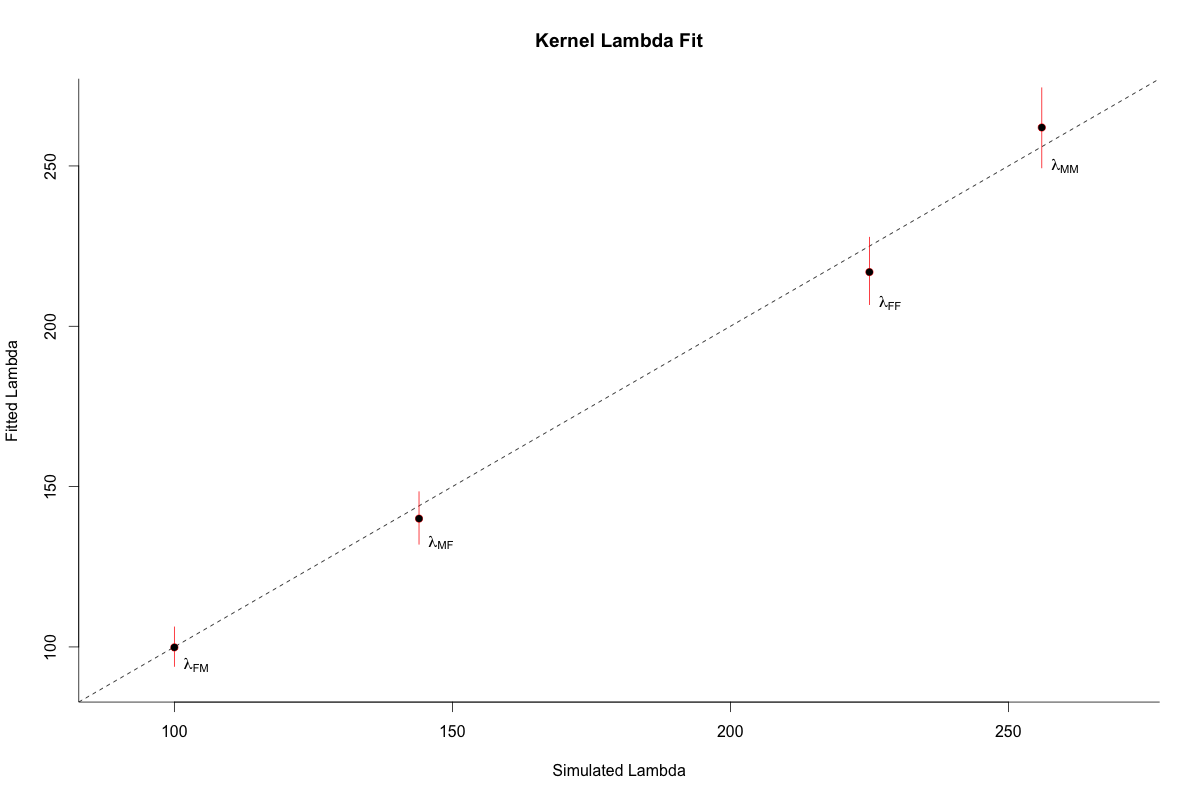
\includegraphics[scale = 0.39]{Lambda_Estimates.png}

\pagebreak
\noindent The degrees are also recovered well, with a correlation of 0.98 between the simulated values and their posterior means.

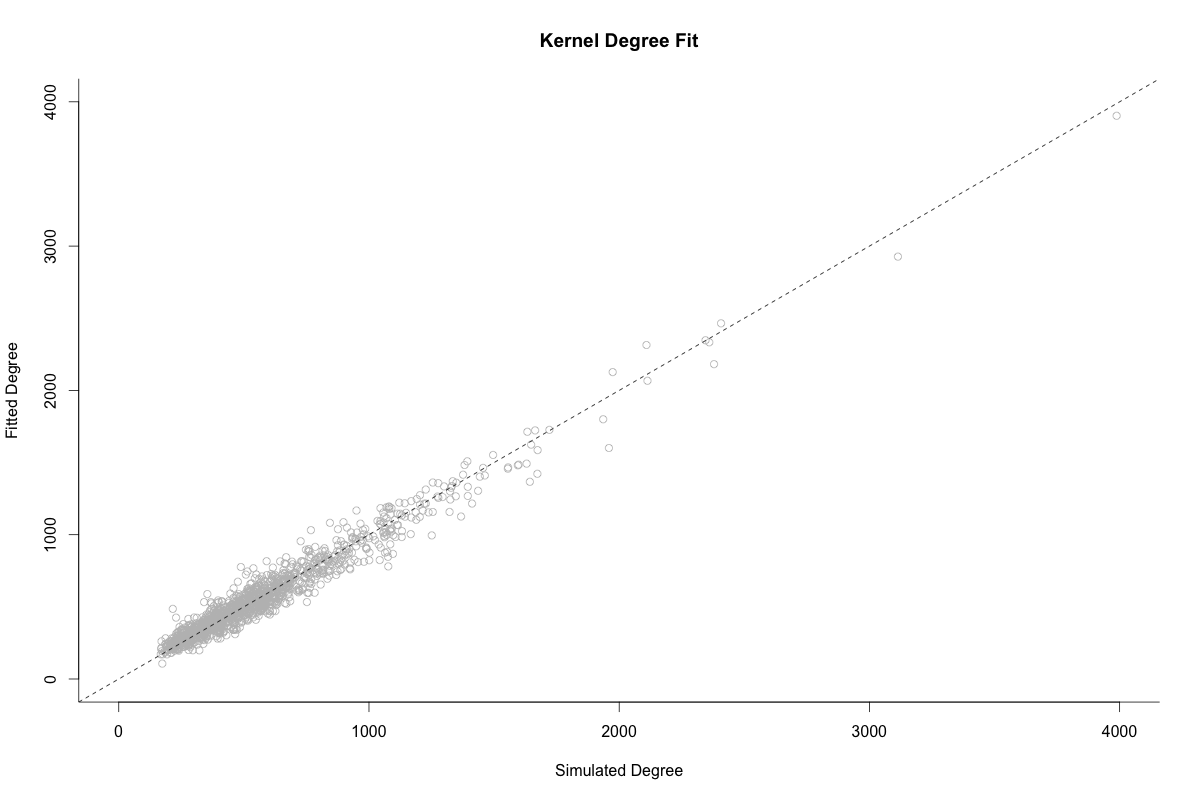
\includegraphics[scale = 0.38]{Degree_Estimates.png}

\noindent The overdispersions are also mostly contained within the central 95\% of their posterior distributions, but posterior uncertainty is quite large. Here the posterior median is preferred to the posterior mean.

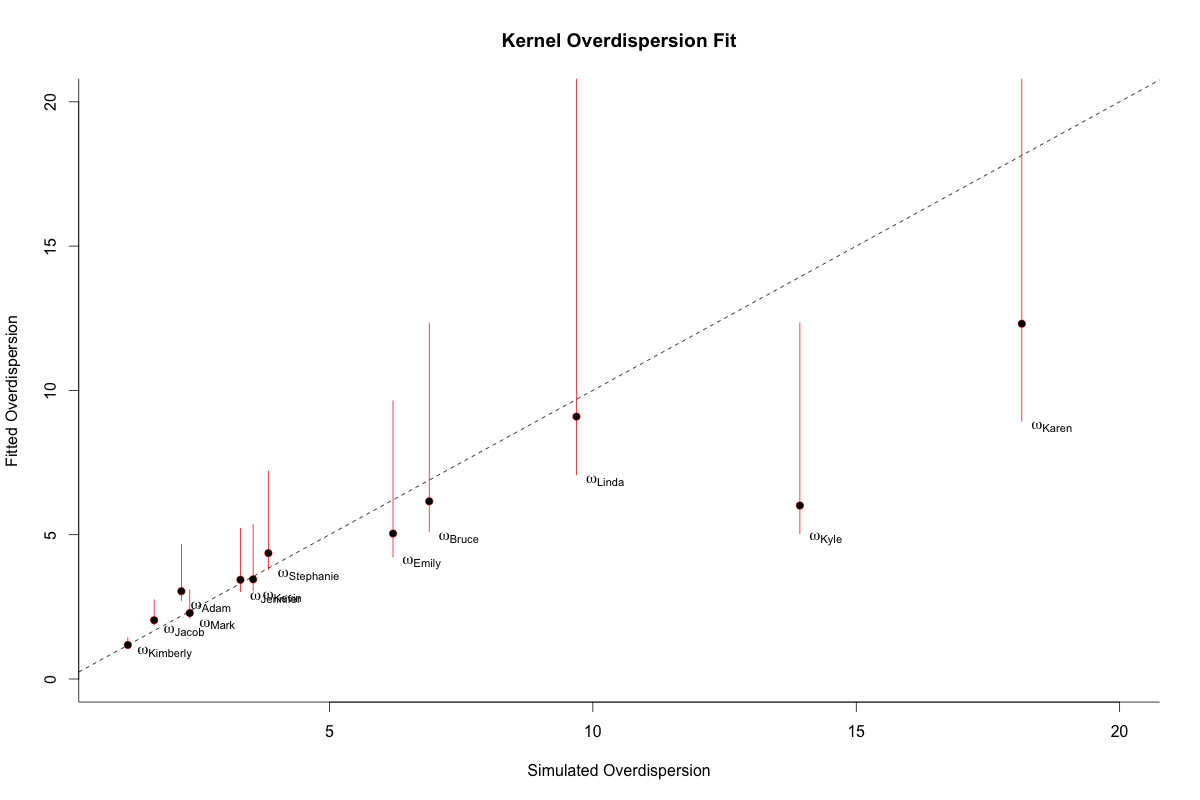
\includegraphics[scale = 0.38]{Overdispersion_Estimates.png}

%JUSTIFICATION%
\pagebreak
\subsection*{Issues}
One of the major assumptions is that the age distribution, conditional on name and gender, is an unconstrained normal. However we see that this assumption is violated by many of the names in the actual data. Some name distributions have multiple modes while others are clearly truncated.

\noindent 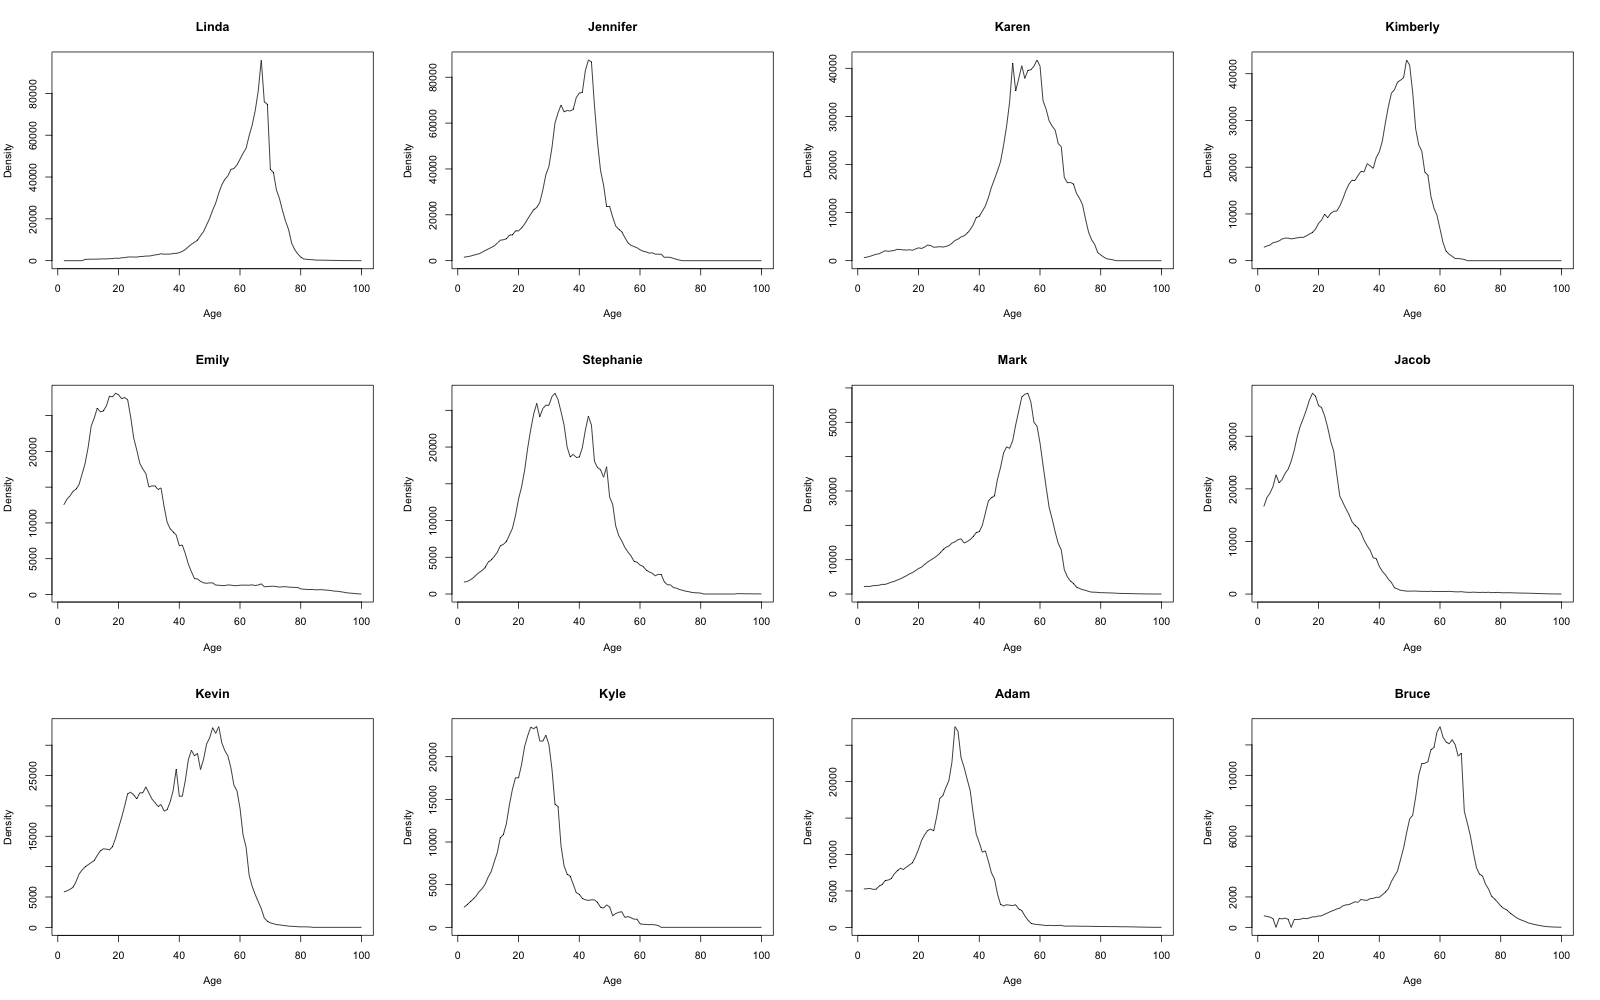
\includegraphics[width=\textwidth]{Name_Age_Histograms.png}

\noindent Additionally, the assumption that the kernel is an unconstrained Gaussian would likely be unrealistic for egos with ages close to 0 or 100 (for the same truncation reason it is violated for alter groups like Emily above). Lastly, our kernel does not allow multi-modality (for example, the kernel doesn't allow peaks around ages of grandparents and around the ages of children).

\end{document}